\chapter{Metodología}\label{chap:metodologia}
En este capítulo se detallan los diferentes procesos en el desarrollo del software que se llevaron a cabo para la realización de la tesis, es decir cuales fueron las diversas etapas que se debió realizar y cual fue su organización.

\begin{center}
\begin{minipage}{0.8\linewidth}  \vspace{5pt} {\small
Una metodología en el desarrollo se refiere al entorno que se usa para estructurar, planificar y controlar el proceso de desarrollo de un sistema de información. Este proceso es un conjunto de actividades que conducen a la creación de un producto .}
\begin{flushright}
  \citep{sommerville}
\end{flushright}
\end{minipage}
\end{center}

El modelo utilizado para el desarrollo de esta tesis está en función de los objetivos planteados en el Capítulo \ref{chap:introduccion}. La misma se dividió en diferentes fases, siguiendo un modelo de desarrollo incremental e iterativo.

En los siguiente ítems se describirán las diferentes fases que se llevo a cabo para alcanzar el objetivo planteado en el desarrollo de la tesis:
\begin{itemize}
	\item \textbf{Fase 1: Investigación de la temática de estudio}\\
	En esta fase se realizó la búsqueda bibliográfica relacionada a la temática de estudio (visión artificial, detección de objeto, 
	Aprendizaje Profundo, Aprendizaje Automático, imágenes satelitales, librerías de desarrollo, métodos de clasificación y regresión).
	\item \textbf{Fase 2: Preparación e Instalación de entorno de Desarrollo.}\\
	En esta fase se realizó la instalación de las herramientas y librerías necesarias para el desarrollo del software; se instalaron librerías  
como(Keras, SkLearn, Python-libs, entre otras).
	\item \textbf{Fase 3: Análisis e Diseño del Software.}\\
	Se analizaron diferentes técnicas de \ac{va} y \ac{ml} para ser implementadas. En esta fase también se recopilo los \textit{datasets} (conjunto de datos) para el desarrollo.
	\item \textbf{Fase 4: Desarrollo y Evaluación de resultados.}\\
	En esta fase se realizo la evaluación experimental de los datos obtenidos, optimizando los diferentes parámetros para la obtención de un 
modelo mas eficiente.
	\item \textbf{Fase 5: Escritura de Informe y Conclusiones.}\\
	Para finalizar se realizó la escritura de la tesis además se elevaron las conclusiones del desarrollo, evaluando lineas futuras de trabajo.
\end{itemize}

% \section{Requerimientos del Software}\label{sec:requerimientos}

% En la siguiente (tabla: \ref{tab:tabladerequerimiento}), se enumeran las especificaciones de requerimiento en el desarrollo del software. 
% \begin{table}[H]
% 	\begin{center}
% 	\begin{tabular}{|c|p{9cm}|c|}\hline
% 		\rowcolor[gray]{0.9} \textbf{\large ID} & \centering \textbf{\large Requerimientos} &\textbf{\large Tipo}\\
% 		\hline
% 		0 & El sistema deberá detectar un área de interés en una imagen satelital &Funcional\\\hline
%         2 & La imágenes deberá tener las bandas TBD del espectro visible & TBD\\\hline
%         3 & El software usará técnicas de Machine Learning para el procesamiento de la imágen satelital & Funcional	\\\hline
%         4 & EL software usará técnica de Computer Vision para el procesamiento de la imágen satelital. & Funcional \\\hline
%         5 & Se deberá contar con datos de entrada para su simulación: un conjunto de imágene, datos de coordenadas de los puntos de interés & Funcional	\\\hline
%         6 & El software deberá ser implementado en un lenguaje de programación que soporte tecnología de ML y VA & TBD	\\\hline
%         7 & El software deberá ser documentado  & TBD	\\\hline
%         8 & El software medirá el tiempo de procesamiento de las técnicas a usar  & TBD	\\\hline
%        	9 & El software deberá hacer un pre-procesamiento de la imágen  &	TBD\\\hline
% 	\end{tabular}
%     \caption{Requerimientos de Software} \label{tab:tabladerequerimiento}
%     \end{center}
% \end{table}

\section{Contexto del Sistema}\label{sub:casodeuso}

En la siguiente figura (ver: \ref{Fig: diagbloque}), se muestra el diagrama de bloque del sistema, donde observamos la arquitectura general del software. 

\begin{figure}[H]
 \centering
  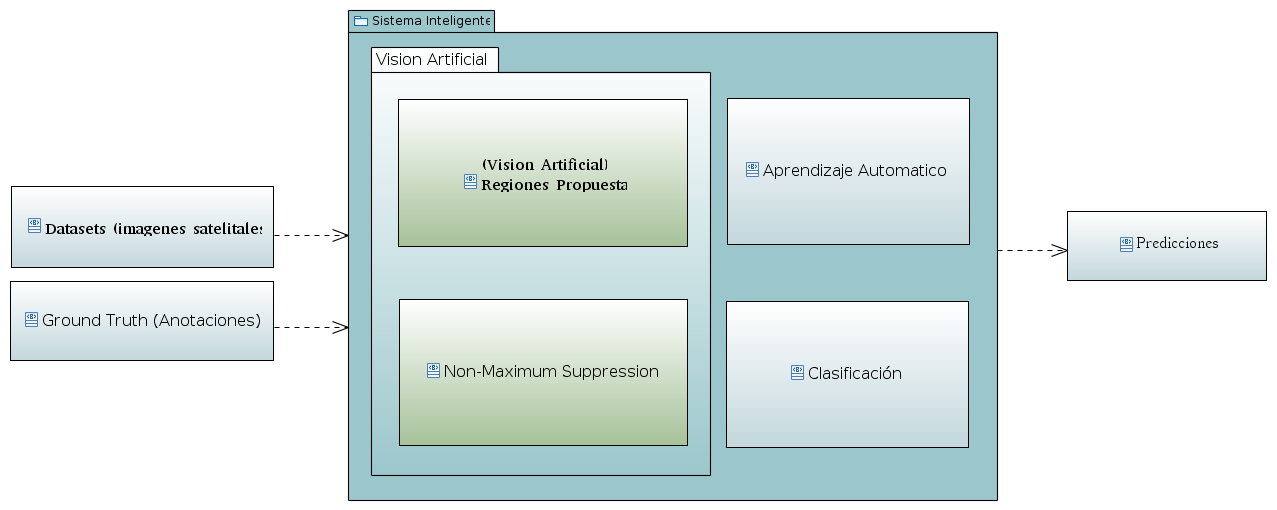
\includegraphics[height=7cm,keepaspectratio=true,clip=true]{imagenes/Logos/diagramabloque.png}
  \caption{Arquitectura del Software de reconocimiento}
	\label{Fig: diagbloque}
 \end{figure}
